
\section{Introduction} % Sections are added in order to organize your presentation into discrete blocks, all sections and subsections are automatically output to the table of contents as an overview of the talk but NOT output in the presentation as separate slides

%------------------------------------------------

\begin{frame}
\frametitle{FoundationDB}

\begin{figure}
    \centering
    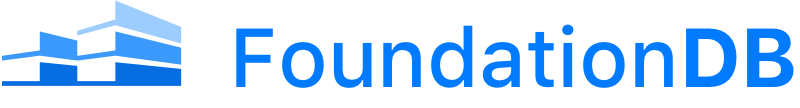
\includegraphics[width=0.5\textwidth]{img/1-Introduction/foundationBD-logo.png}
    
\end{figure}

\textbf{FoundationDB}FoundationDB is an open-source transactional key-value store created by Apple in 2009. It combine \textbf{flexibility} and \textbf{scalability} of \textbf{NoSQL} architectures with the power of \textbf{ACID transactions}.
	
\end{frame}

%------------------------------------------------

\begin{frame}
	\frametitle{FDB Key features}

Key features:
\begin{itemize}
    \item NoSQL
    \item Ordered
    \item strictly serializable transactions
    \item ACID transactions
    \item Flexible and Scalable
    
\end{itemize}

\end{frame}
%------------------------------------------------
\begin{frame}
	\frametitle{CAP trade off}

A tradeoff exists between consistency, availability, and
partition tolerance
\begin{itemize}
    \item Consistency: A read sees all previously completed writes
    \item Availability: Reads and writes always succeed
    \item Partition tolerance: Guaranteed properties are maintained even when network failures prevent some machines from communicating with others.
    
\end{itemize}
FoundationBD satisfied \textbf{Availability} and \textbf{Partition Tolerance} 

\end{frame}
%------------------------------------------------
\begin{frame}
	\frametitle{CAP Theorem Examples}

\begin{figure}[h]
    \centering
    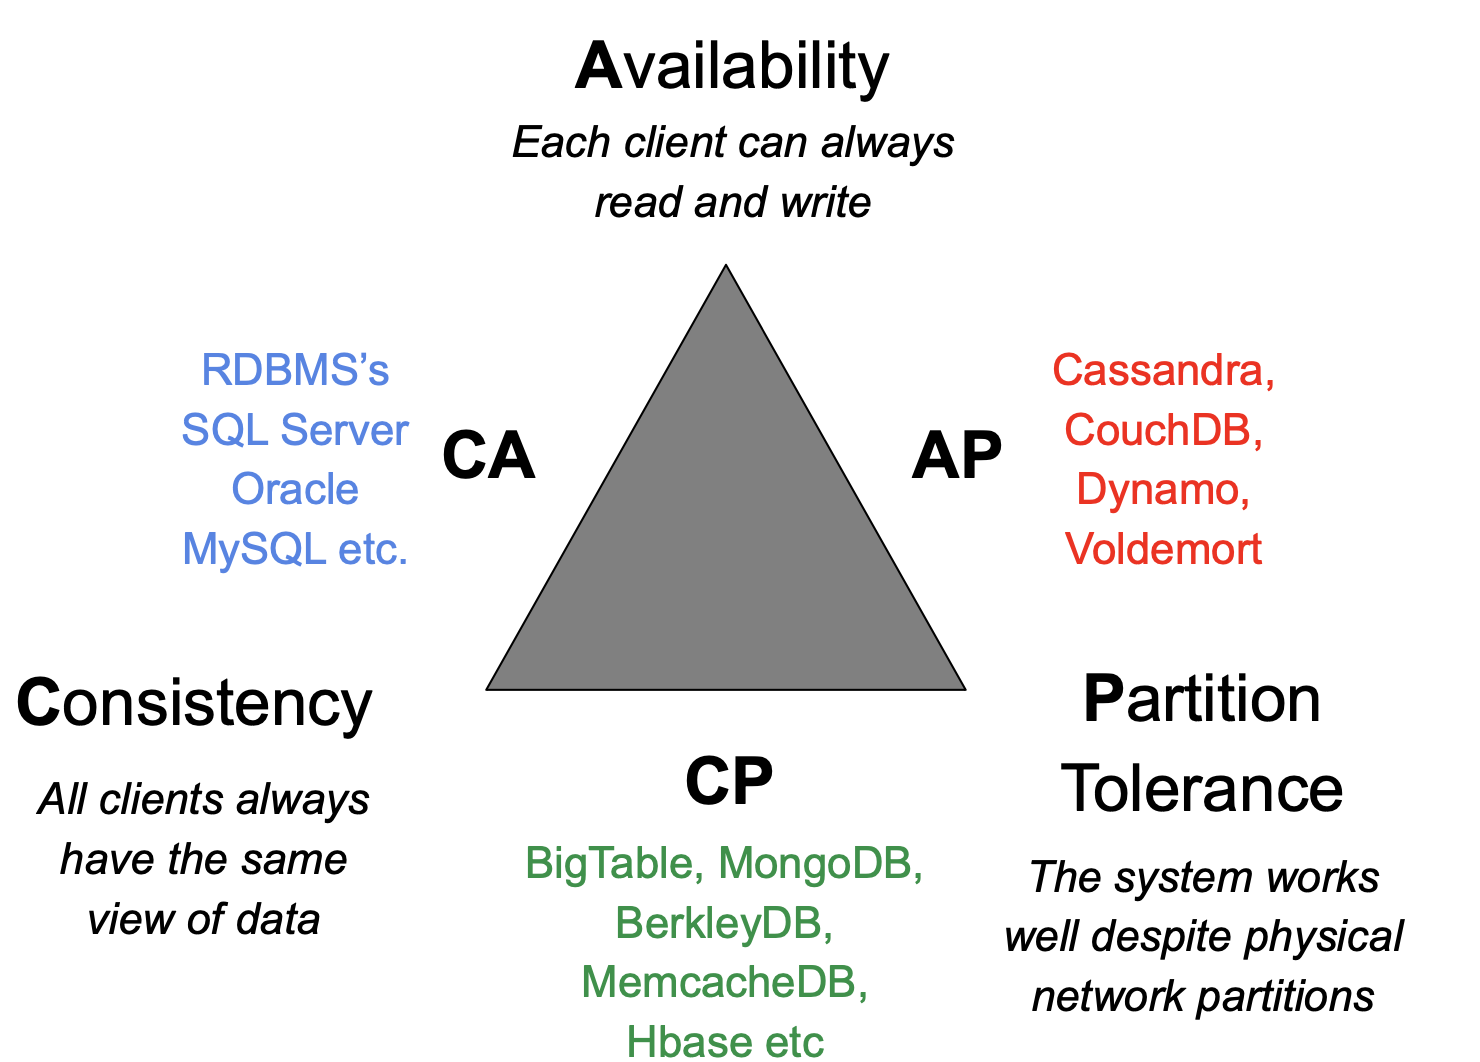
\includegraphics[width=0.7\textwidth]{img/1-Introduction/CAP theorem.png}
    \caption{CAP Theorem (or triangle)}
\end{figure}

\end{frame}

%------------------------------------------------

\begin{frame}
	\frametitle{Consistency over Availability}

 Availability in the CAP sense means that all nodes remain able to read and write even when partitioned. A system that keeps some, but not all, of its nodes able to read and write is not Available in the CAP sense, even if it remains available to clients and satisfies its SLAs for high availability.
\vspace{0.5cm}

As any ACID database must, during a network partition FoundationDB chooses Consistency over Availability. 

\end{frame}

%------------------------------------------------

\begin{frame}
	\frametitle{FoundationDB approach}
Most database: 
    \begin{itemize}
        \item Storage engine
        \item Data model
        \item API/Query language
    \end{itemize}

FoundationDB has a modular approach, it it provides a highly scalable storage engine with a minimal yet carefully chosen set of features.

\vspace{0.5cm}
\begin{quote}
    "What features could we take away? Almost everything, we decided."
\end{quote}
        
\end{frame}


%------------------------------------------------

\begin{frame}
	\frametitle{Less is more: The FoundationDB way}
FoundationDB decouples its data storage technology from its data model. FoundationDB’s core ordered key-value storage technology can be efficiently adapted and remapped to a broad array of rich data models.
\end{frame}

%------------------------------------------------

\begin{frame}
	\frametitle{Example: indexing}

FoundationDB’s core provides no indexing.
Instead, a layer provides indexing by storing two kinds of key-values, one for the data and one for the index.

\begin{center}
\textcolor{red}{people/alice/eye\_color = blue}
\end{center}
\begin{center}
\textcolor{red}{eye\_color/blue/alice = true}
\end{center}

ACID transactions allows to update both the data and the index in a single transaction.
\end{frame}

%------------------------------------------------

\begin{frame}
	\frametitle{Layer strategy}

Popularity and growing open source community is FoundationDB’s focus on the “lower
half” of a database, leaving the rest to its “layers”.

Examples:
\begin{itemize}
    \item \textbf{FoundationDB Record Layer}: adds back much of what users expect from a relational database
    \item \textbf{JanusGraph}: graph database
    \item \textbf{CouchDB}
\end{itemize}
\end{frame}


%------------------------------------------------

\begin{frame}
	\frametitle{What will be discussed in the next chapters}

    \begin{itemize}
        \item Architecture of FoundationDB
        \item Simulation and Testing of distributed system
        \item Evaluation of FoundationDB
        \item Conclusions
    \end{itemize}
        
\end{frame}

%------------------------------------------------

